\chapter{Experimental setup}
This chapter provides a description of the experimental setup used to evaluate the clustering aggregation protocol in different quantum computing environments, both on a simulator and on real hardware. The protocol was tested on three distinct platforms: a simulator for a neutral atom quantum computer, specifically the Pulser simulator by PASQAL; the Fresnel neutral atom quantum computer, also developed by PASQAL; the Advantage quantum annealer with Zephyr topology, developed by D-Wave.

\section{Dataset}
The dataset used to test the protocol is shown in figure \ref{fig:dataset}. It is specifically designed to contain different shapes and configuration of points that  

It was first introduced by Gionis, Mannila and Tsaparas to test classical clustering aggregation algorithms \cite{dataset}; it was then used by Li and Latecki to test a clustering aggregation protocol that uses simulated annealing \cite{aggregation}. 

\begin{figure}[ht]
  \centering 
  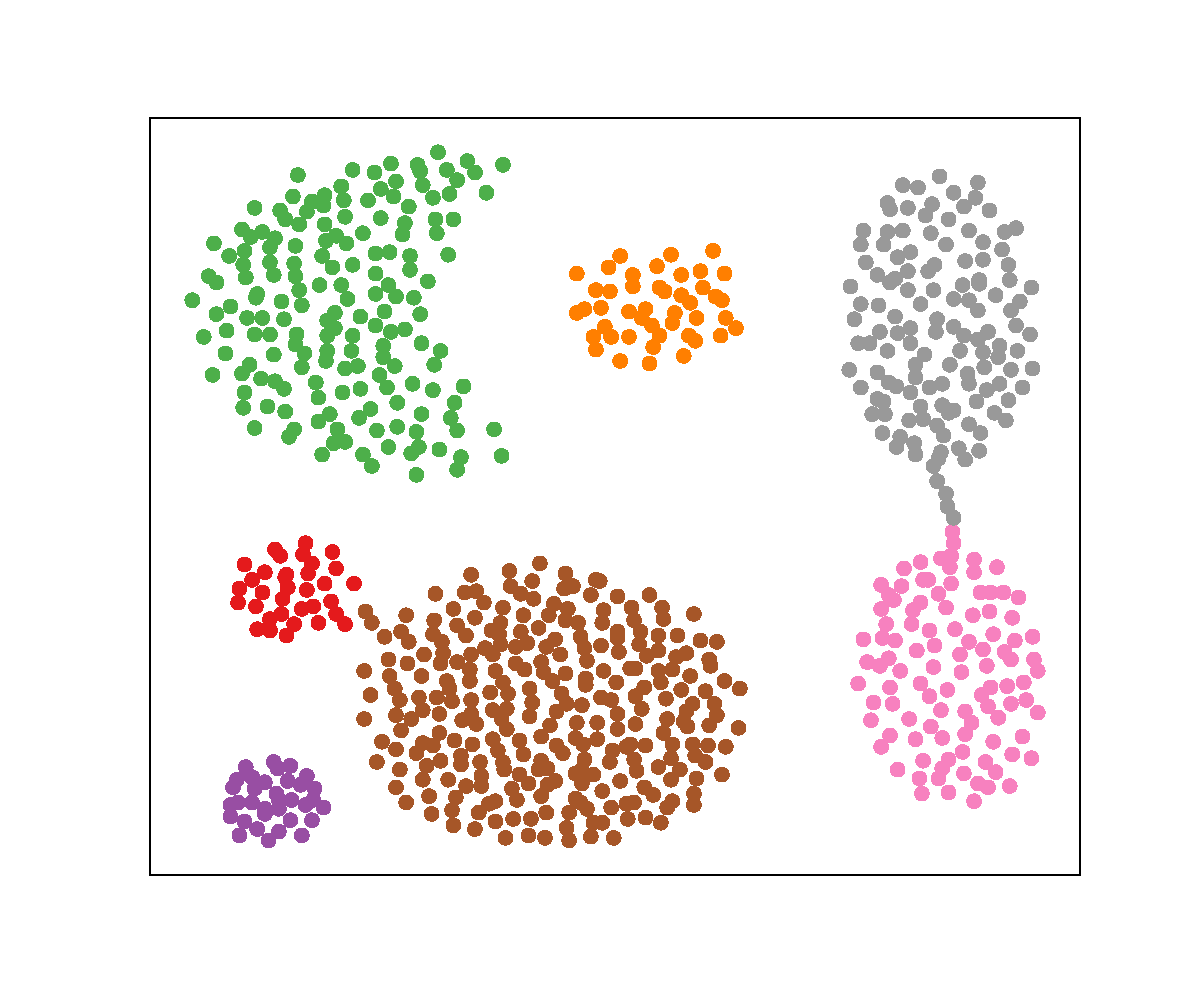
\includegraphics[width=0.9\textwidth]{figures/03experimental_setup/dataset.pdf}
  \caption{Dataset plot}
  \label{fig:dataset}
\end{figure}

\section{Evaluation metrics}
Different metrics were used to evaluate the quality of single clusters and of clustering algorithms as a whole. Silhouette score was used as the criterion to 

\subsection{Silhouette score}
The silhouette score is a metric used to evaluate clustering quality, introduced by Peter J. Rousseeuw \cite{Rousseeuw1987}. The score is computed for each point in the dataset and reflects both its cohesion with points in the same cluster, as well as the separation with respect to points in different clusters. Specifically, the silhouette score of a point $p$ in the dataset is defined as 
\begin{equation}
  \label{eqn:silhouette}
  S_{p} = \frac{b_{p} - a_{p}}{\max({a_{p}, b_{p}})},
\end{equation}
where $a_{i}$ is the average distance from the point to other points in the same cluster (intra-cluster distance), and $b_{i}$ is the average distance to points in the nearest different cluster (inter-cluster distance). The score ranges between -1 and 1, where values close to 1 indicate that points are well-clustered, with high cohesion and good separation, while negative values suggest points may have been assigned to the wrong cluster. 

A quantification of the quality for a single cluster can be obtained by computing the average of the silhouette score; more formally, for a cluster $c_{i}$, the formula for its average silhouette ($AS_{i}$) is 
\begin{equation}
  \label{eqn:cluster_silhouette}
  AS_{i} = \frac{\sum_{p \in c_{i}} S_{p}}{|c_{i}|}
\end{equation}
